%% LyX 2.0.3 created this file.  For more info, see http://www.lyx.org/.
%% Do not edit unless you really know what you are doing.
%\documentclass[english]{article}
%\usepackage[T1]{fontenc}
%\usepackage[latin9]{inputenc}
%\usepackage{graphicx}
%\usepackage{babel}
%\begin{document}

\section{GUI Design and Implementation}
\label{guidesign}

The target userbase for the evacuator does not guarantee a good degree
of computer-literacy. Hence a clear and easy to use GUI was required.


\subsection{Initial Design}

Based from initial system requirements a wireframe for the GUI could
be generated. To keep the user experience simple it was decided to
keep all the basic functionality within the main window. This allows
unfamiliar users to gain from the software without being overwhelmed
by endless options. For advanced configuration there was to be a detailed
configuration panel allowing advanced users to set the majority of
variables as they saw fit.

The wireframe below was drawn up to support these concepts. By sticking
to conventions it gives a familiar feel to most who have used a typical
windows based system within the last decade.\\

\begin{figure}
\centering
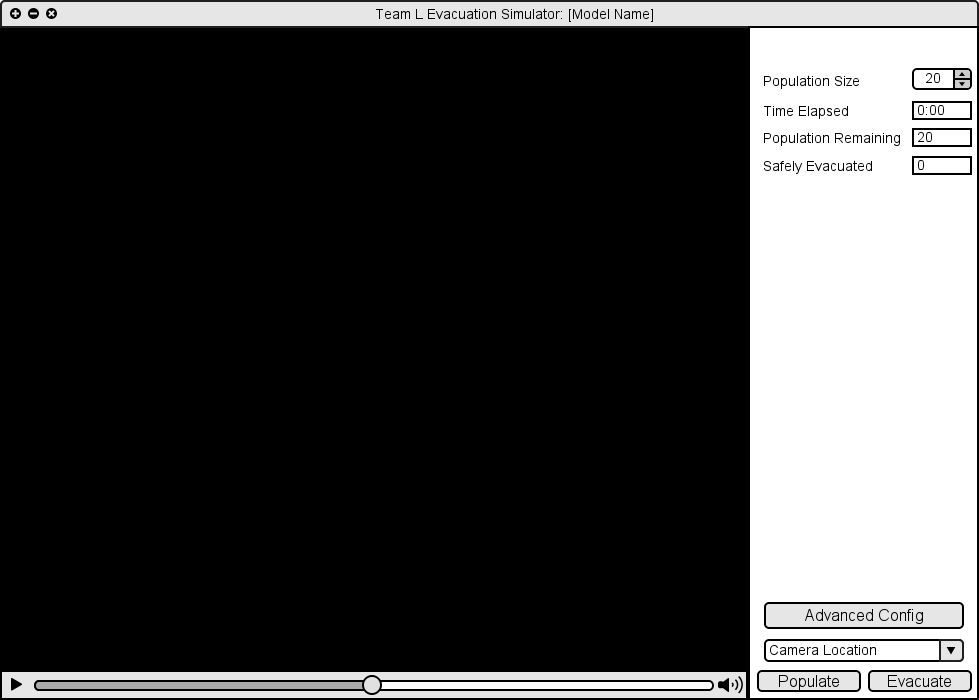
\includegraphics[width=10cm]{../images/GUIv1WF}
\caption{First attempt at wireframing GUI\label{ref:initialGUI}}
\end{figure}

%\caption{Sample configuration\label{fig:sampleconfig}}

\subsection{GUI Implementation and Revision}

It was decided since the project was to be built in Java and several
members had knowledge of the library to use Swing for implementation
of the GUI. The toolkit was more than capable of our needs and any
advantages of alternatives seemed unlikely to counterbalance the time
required to learn a new environment. SWT was briefly considered since
the interface created generally allows a closer to native feel and
higher performance \cite{SWT}.
This however would come at a cost of portability as well as the time
consideration mentioned above.

The initial GUI implementation (\ref{ref:initialGUI}) was a quick and crude attempt towards the initial
wireframe. Its purpose was more towards checking how well the JMonkey
canvas could be displayed within the Swing layout than producing a
suitable end product.\\

\begin{figure}
\centering
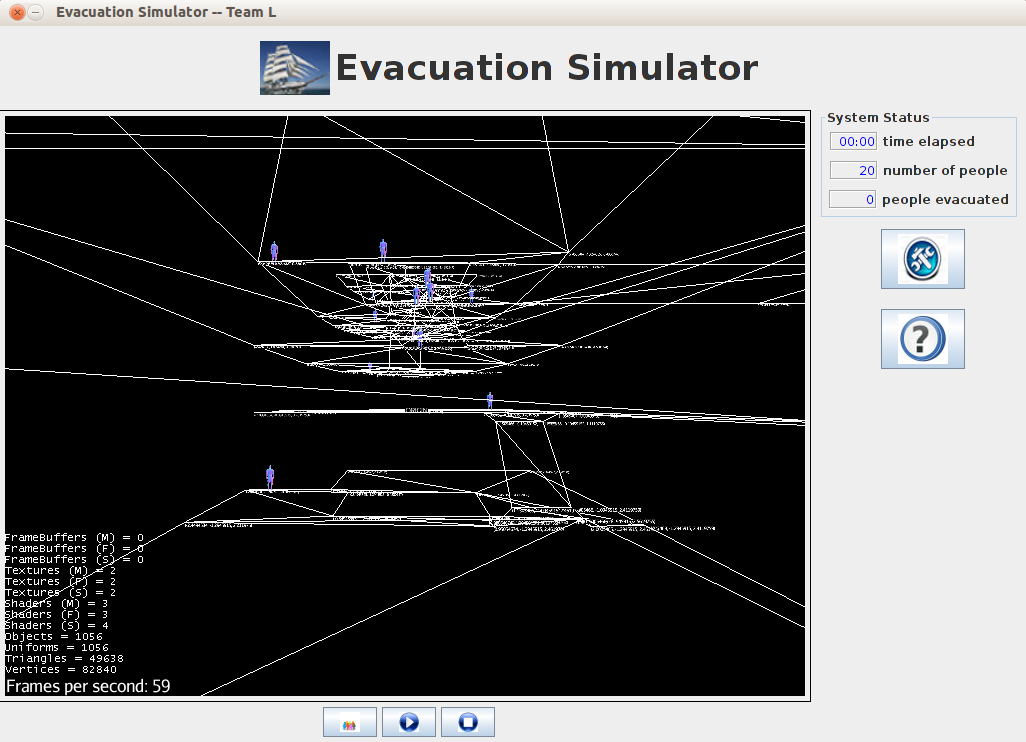
\includegraphics[width=10cm]{../images/GUIv1}
\caption{First refinement of GUI}
\end{figure}

Whilst not particurly attractive a suitable platform for basic testing
was then available.

At this point it became apparent that the back end would not easily
allow for the evacuation to be ``scrolled through'' in the way we
had initially anticipated. The play bar at the bottom of the screen
was removed from designs. this led to the control buttons being moved
to the panel on the right. After speaking to some less computer-literate
users it was further decided to use a traditional menu-bar. Some also
found the navmesh didn't give an immediate understanding of what
the model represented so toggles were added to allow a physical representation
of the ship to be shown.

These changes manifested themselves as can be seen in \ref{secondRefinementGUI}. Due to more
time being spent on this iteration it gives a much more complete feel
and is considerably closed to the initial wireframe.\\

\begin{figure}
\centering
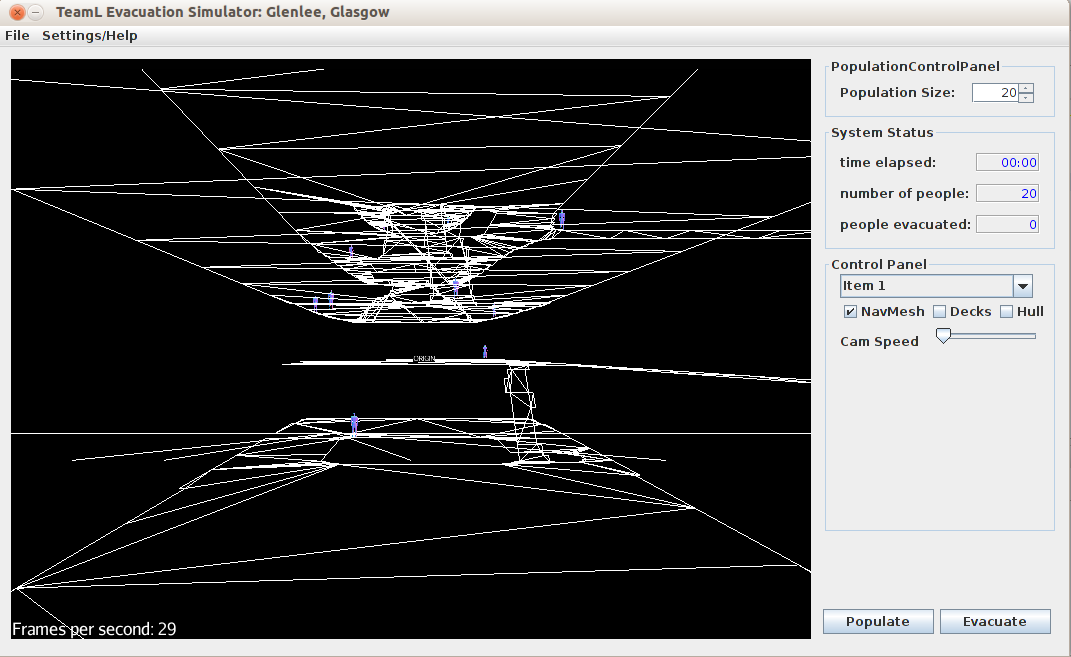
\includegraphics[width=10cm]{../images/GUIv2}
\caption{Second refinement to GUI\label{secondRefinementGUI}}
\end{figure}

Further talks with users suggested that for those not used to computer-games
the keyboard based camera controls were not immediately understandable.
To fix this a control panel was added. Due to the way functionality was implemented
a route button was added for testing purposes. It was then decided
this would be of use to users so was left in. Finally, to allow a
more native feel the theming was set to inherit from the system the
code was run from. A new wireframe (\ref{thirdRefinementGUI}) was drawn up  to
show this.\\

\begin{figure}
\centering
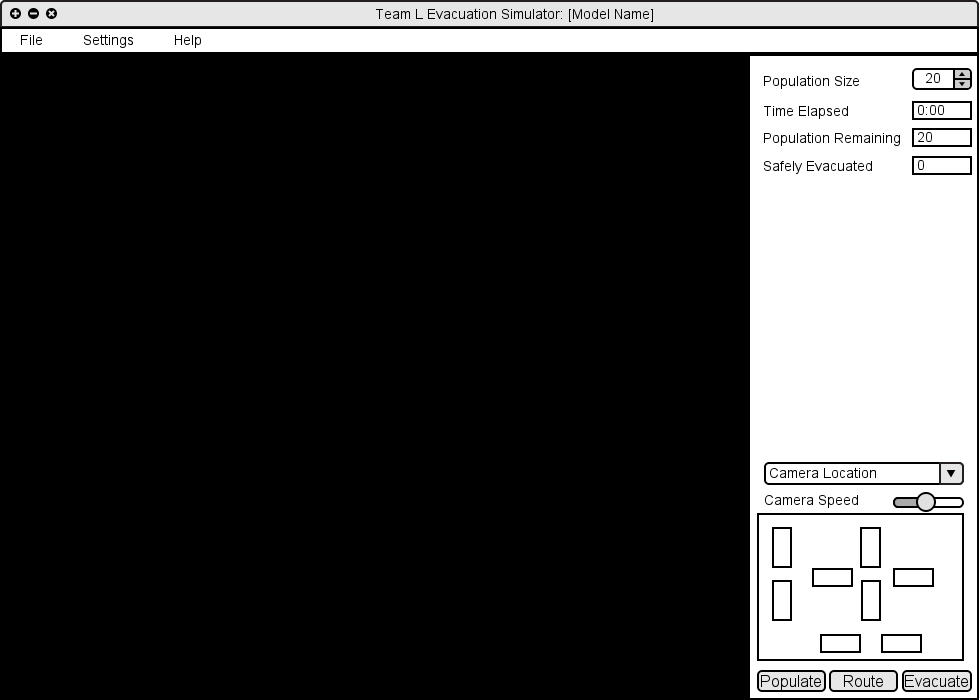
\includegraphics[width=10cm]{../images/GUIv2WF}
\caption{Third refinement to GUI\label{thirdRefinementGUI}}
\end{figure}

\subsection{Final GUI}

The wireframe in \ref{finalGUI1} was implmented to give our final GUI. It gives
a polished finish and meets original aims well and takes into consideration
user feedback. 

Initial work was done using the Netbeans GUI builder. This allowed
the layout we required to be built quickly, but not the functionality.
To achieve this some work was needed on the raw swing code.

The final interface is shown in \ref{finalGUI2}, both in Linux and Windows.\\

\begin{figure}
\centering
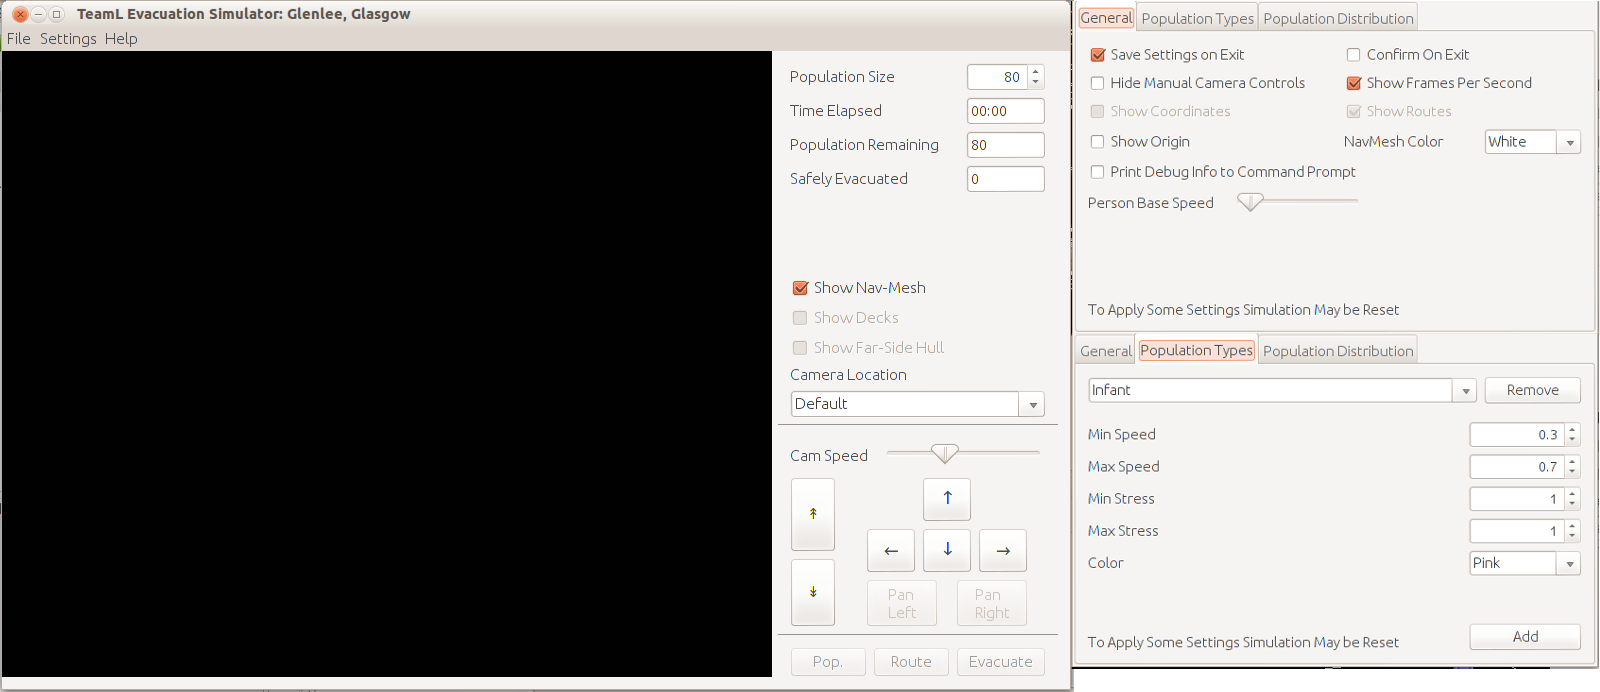
\includegraphics[width=18cm]{../images/GUIv3FULL}
\caption{Final GUI wireframe\label{finalGUI1}}
\end{figure}

\begin{figure}
\centering
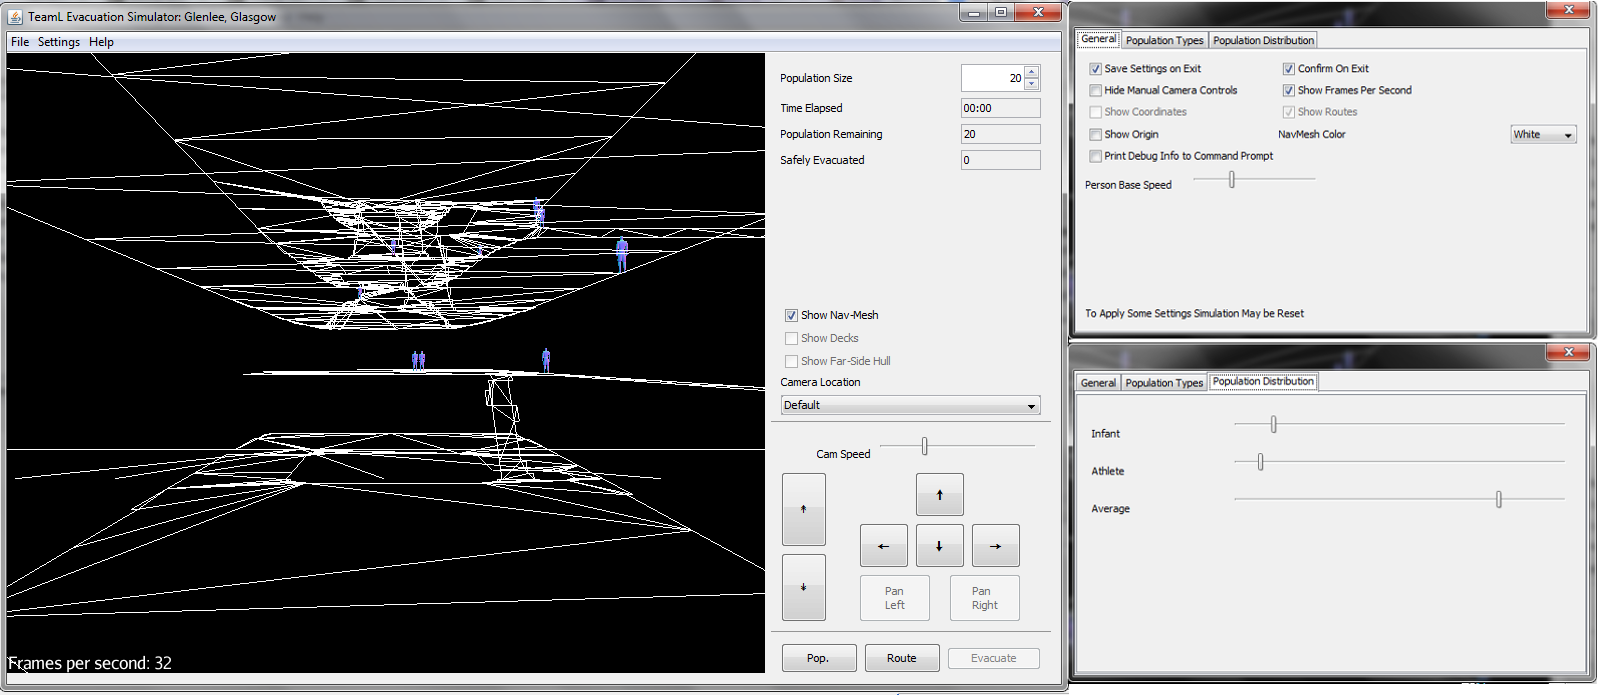
\includegraphics[width=18cm]{../images/GUIv3FULLWIN}
\caption{Final GUI in Swing\label{finalGUI2}}
\end{figure}


%\end{document}
